\chapter{Objetivos}\label{cap.Objetivos}
Una vez presentado el contexto de este TFM en el primer capítulo, yendo de lo más general (tipos de clasificadores) a lo más cercano (el clasificador a utilizar), en este capítulo se van a explicar los objetivos concretos a conseguir y la metodología utilizada para llegar a ello.

\section{Objetivo principal}
El objetivo principal es hacer funcionar BAdaCost detector, desarrollado para matlab, en C++. Para ello, utilizando la misma imagen de entrada y el mismo detector, hay que obtener la misma salida (mismas detecciones o muy parecidas). Para llegar a esto, se han propuesto distintas fases:

\begin{itemize}
\item \textbf{Extracción de características: } Para poder clasificar bien los elementos de las imágenes, hay que extraer de forma correcta las características. En este caso los detectores trabajan con diferentes características (espacios de color, magnitud del gradiente y magnitud del histograma). Por ello, se realiza el desarrollo para C++, comparando siempre que los resultados obtenidos sean los mismos que en Matlab.

\item \textbf{Procesamiento de las características: } Una vez se realiza la extracción de características, pueden darse distintos procesos de transformación como redimensionados, suavizados o relleno (padding) sobre lo obtenido. El siguiente paso era asegurar que estos procesos retornan también el mismo resultado en C++ que en Matlab.

\item \textbf{Realizar la detección: } Una vez se tienen las características procesadas igual que en Matlab, lo siguiente es realizar la detección. Para ello, hay que guardar el detector de Matlab en un formato legible en C++, leer los parámetros del detector y poder utilizarlos correctamente. Una vez se pueden cargar los parámetros del detector, desarrollar el algoritmo de detección en C++.
\end{itemize}


\section{Requisitos}
Para la realizaci\'on de los objetivos anteriormente citados, se tiene que conseguir una soluci\'on que cumpla las siguientes caracter\'isticas:
\begin{itemize}
\item Que se trate de un algoritmo robusto, capaz de trabajar con distintos clasificadores y que no dependa de unos parámetros determinados, sino que sea capaz de obtener resultados óptimos en distintos casos.

\item Que el algoritmo sea capaz de trabajar en distintos tipos de máquinas, no necesitando unas características específicas, solo que permita ejecutar C++ y tenga la librería OpenCV instalada.

\end{itemize}

\section{Metodolog\'ia}

La metodología propuesta es un desarrollo en espiral. Para ello se proponen semanalmente reuniones con el tutor, en las cuales se presentaba lo conseguido en el último periodo en relación a los objetivos propuestos y se proponían los nuevos objetivos para la siguiente reunión. Sobre las tareas propuestas se evaluaban los riesgos que podían darse y los avances que se conseguirían en función del camino tomado. Después, se continuaba desarrollando el algoritmo para conseguir los objetivos.Se probaba en todo momento mediante tests si lo desarrollado funcionaba o no. En función del resultado de estos tests, se determinaba si el objetivo se había conseguido o no. Si no se conseguía, analizar el fallo para solventarlo. En caso de que se consiguiese o estar cerca, se proponían nuevos objetivos para continuar con el trabajo.

\begin{figure}[H]
	\centering
		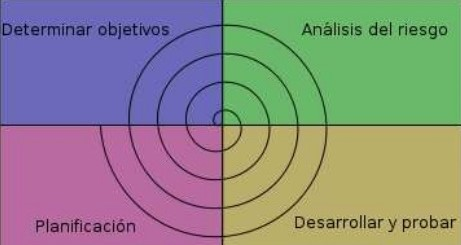
\includegraphics{imgs/metodologia-espiral.jpg}
        \caption{M\'etodo de desarrollo en espiral}
	\label{fig:Desarrollo en espiral}
\end{figure}

Durante todo el desarrollo, se utilizado GitHub como repositorio del código, explicando cuales eran los últimos avances subidos en los \textit{commits} y generando un \textit{issue} por cada tarea a realizar, poniendo en él las diferentes dudas que surgían e indicando la resolución final. De esta forma, se conseguía un desarrollo y una comunicación fluida, quedando el código públicamente accesible en \href{https://github.com/RoboticsURJC-students/2017-tfm-jorge_vela}{https://github.com/RoboticsURJC-students/2017-tfm-jorge_ vela}.



\section{Plan de trabajo}
La planificación seguida en el desarrollo ha incluido las siguientes fases:

\begin{itemize}
\item{Investigación: }Comprender el funcionamiento del \textit{toolbox} de badacost, ver la organización del código y su funcionamiento, tanto de las funciones por separado como el algoritmo en conjunto, para ver la extracción de características y el funcionamiento del conjunto final.

\item{Desarrollo del código: } Una vez visto el funcionamiento, trabajar en el código para que BAdaCost funcionara en C++ de forma robusta. Para ello, por cada clase o función que se creaba, se realizaba un test de prueba. Con esto, cuando se obtiene el resultado de C++ se compara con el de Matlab, de forma que se asegura un resultado correcto. Los tests también ayudan si a lo largo del desarrollo, se produce algún cambio en el código. Al comprobar continuamente que todo lo anterior funciona, si un cambio provoca fallo es muy fácil de detectar y saber porque ocurre.

\item{Compatibilidad entre Matlab y C++: } Bien sea para comparar los datos, o para utilizar el mismo detector, tiene que haber un método que permita tener datos iguales en ambos lenguajes. Para ello se ha utilizado el formato YML. Con esto, se pueden guardar todo tipo de datos desde matlab (como el resultado de funciones determinadas o los parámetros de un detector) y leerlo desde C++.
En Matlab se ha creado una función que guarda lo deseado con un formato determinado, el cual se lee desde el código desarrollado en C++.  

\end{itemize}






























